\subsection{WebSocket}

\begin{frame}{WebSocket}{Applikationsprotokolle}
  \begin{center}
    \begin{figure}
      \par\bigskip
      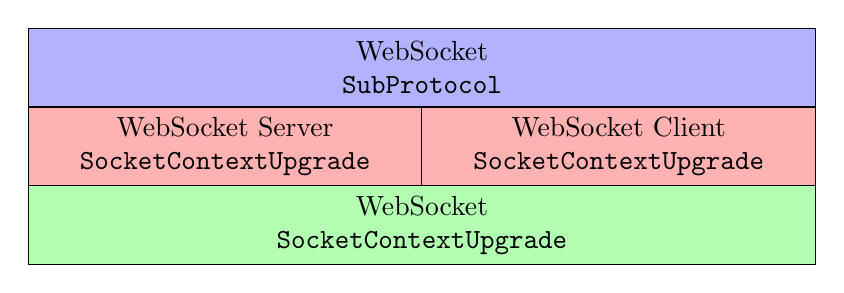
\begin{tikzpicture}
        \draw node [outer sep=0, inner sep=0, draw, fill=green!30, minimum width=10cm, minimum height=1cm, align=center] (wstr) {WebSocket\\\texttt{SocketContextUpgrade}};
        \draw (wstr.north) node[anchor=south west, outer sep=0, inner sep=0, fill=red!30, draw, minimum width=5cm, minimum height=1cm, align=center] (wsc) {WebSocket Client\\\texttt{SocketContextUpgrade}};
        \draw (wstr.north) node[anchor=south east, outer sep=0, inner sep=0, fill=red!30, draw, minimum width=5cm, minimum height=1cm, align=center] (wss) {WebSocket Server\\\texttt{SocketContextUpgrade}};
        \draw (wss.north east) node[anchor=south, outer sep=0, inner sep=0, fill=blue!30, draw, minimum width=10cm, minimum height=1cm, align=center] (sp) {WebSocket\\\texttt{SubProtocol}};
      \end{tikzpicture}
      \caption{WebSocket-Applikationsprotokoll im Detail}
    \end{figure}
  \end{center}
  \begin{itemize}
    \item Die WebSocket Libraries werden bei HTTP-\texttt{upgrade} dynamisch (\texttt{dlopen()}, \ldots) eingebunden.
    \item Anhand des angeforderten \texttt{SubProtocol}s (z.B.  \texttt{tiktaktoe}, \texttt{echo}, \texttt{mqtt}) werden die entsprechenden \texttt{SubProtocol} Libraries dynamisch geladen.
    \item Sowohl WS Libraries als auch Subprotocol (SP) Libraries müssen einer Namenskonvention gehorchen um gefunden werden zu können.
    \item WS sowie SP Libraries müssen \texttt{static} Factory-Factory Funktionen zur Verfügung stellen.
    \item SP Libraries müssen vom Anwender implementiert werden - abstrakte Basisklasse \texttt{SubProtocol}
  \end{itemize}
\end{frame}
